\chapter{Overview\label{chap:3_video_body_tracking_overview}}

\section{Motion Features Overview}

Traditional methods, as well as the architecture presented in Part~\ref{part:two}, typically use single frame appearance cues such as texture patches, edges, color histograms, foreground silhouettes or hand-crafted local features (such as histogram of gradients (HoG)~\cite{Dalal2005}). In Part~\ref{part:three} we will explore the use of \emph{motion-based} features to improve performance of our network architecture, and we will define and make use of many such features. We will show that our results agree with psychophysical experiments~\cite{biologicalmotion}, which have shown that motion is a powerful visual cue that alone can be used to extract high-level information, including articulated pose.

Previous work~\cite{Ferrari08,weiss:sidestepping} has reported that using motion features to aid pose inference has had little or no impact on performance. Simply adding high-order temporal connectivity to traditional models would most often lead to intractable inference.  In Part~\ref{part:three} we show that deep learning is able to successfully incorporate motion features and is able to out-perform existing state-of-the-art techniques. Further, we show that by using motion features alone our method outperforms~\cite{Eichner:2009:BAM,yang11cvpr,sapp11eccv} (see Fig~\ref{fig:flic_results}(a) and (b)), which further strengthens our claim that information coded in motion features is valuable and should be used when available.

We also present a new dataset called {\bf FLIC-motion}, which is the FLIC dataset~\cite{modec} augmented with `motion-features' for each of the 5003 images collected from Hollywood movies.

\chapter{Architecture\label{chap:3_video_body_tracking_archiecture}}

\section{Body-Part Detection Model} 

We propose a simple extension to the model presented in Part~\ref{part:two}: Section~\ref{sec:conv_model}; the input to the network is an RGB image and an additional set of  \emph{motion features}. Therefore, instead of the previous 3 channel input, the new model will now use 4 to 6 features depending on the motion feature used and we investigate a wide variety of motion feature formulations (section~\ref{sec:motionFeats}).  Finally, we will also introduce a simple Spatial-Model to solve a specific sub-problem associated with evaluation of our model on the FLIC-motion dataset (section~\ref{sec:spatialModel}). For Part~\ref{part:three}, we will not use the full graphical model described in Part~\ref{part:two}: Section~\ref{sec:spatialmodel}, but rather we will implement a simplified model in order to better highlight the impact of our chosen motion features.

\subsection{Motion Features}
\label{sec:motionFeats}

Psychophysical experiments~\cite{biologicalmotion}, have shown that motion is very a powerful visual cue for extracting high-level information. In these experiments, the main joints of a human were represented as a single point, thus degrading the appearance of the object to a minimum, ensuring that any recognition must be based solely on motion. They concluded that proximal motion patterns give the human visual system highly efficient information that carry all the essential information needed for immediate visual identification of such human motions.

The aim of this section is to incorporate features that are representative of the true \emph{motion-field} (the perspective projection of the 3D velocity-field of moving surfaces) as input to our detection network so that it can exploit motion as a cue for body part localization. To this end, we evaluate and analyze four motion features which fall under two broad categories: those using simple derivatives of the RGB video frames and those using optical flow features.  For each RGB image pair $f_{i}$ and $f_{i+\delta}$, we propose the following features:

\begin{itemize}
\item RGB image pair - $\left\{f_{i}, f_{i+\delta}\right\}$
\item RGB image and an RGB difference image - $\left\{f_{i}, f_{i+\delta} - f_{i}\right\}$
\item Optical-flow\footnote{We use the algorithm proposed by Weinzaepfel et al.~\cite{deepflow} to compute optical-flow.} vectors - $\left\{f_{i},\operatorname{FLOW}(f_{i}, f_{i+\delta})\right\}$
\item Optical-flow magnitude - $\left\{f_{i},||\operatorname{FLOW}(f_{i}, f_{i+\delta})||_2\right\}$
\end{itemize}

The RGB image pair is by far the simplest way of incorporating the relative motion information between the two frames.  However, this representation clearly suffers from a lot of redundancy (i.e. if there is no camera movement) and is extremely high dimensional.  Furthermore, it is not obvious to the deep network what changes in this high dimensional input space are relevant temporal information and what changes are due to noise or camera motion. A simple modification to this representation is to use a difference image, which reformulates the RGB input so that the algorithm sees directly the pixel locations where high energy corresponds to motion (alternatively the network would have to do this implicitly on the image pair).  A more sophisticated representation is optical-flow, which is considered to be a high-quality approximation of the true \emph{motion-field}. Implicitly learning to infer optical-flow from the raw RGB input would be non-trivial for the network to estimate, so we perform optical-flow calculation as a pre-processing step (at the cost of greater computational complexity).

\subsubsection{FLIC-motion dataset:}
\label{sec:FLICmotion}
We propose a new dataset which we call {\bf FLIC-motion}\footnote{This dataset can be downloaded from \url{http://cs.nyu.edu/~ajain/accv2014/}}. It is comprised of the original FLIC dataset of 5003 labeled RGB images collected from 30 Hollywood movies, of which 1016 images are held out as a test set, augmented with the aforementioned motion features.

We experimented with different values for $\delta$ and investigated the above features with and without camera motion compensation; we use a simple 2D projective motion model between $f_{i}$ and $f_{i+\delta}$, and warp $f_{i+\delta}$ onto $f_i$ using the inverse of this best fitting projection to approximately remove camera motion. A comparison between image pairs with and without warping can be seen in~Fig~\ref{fig:warpdemo}.
\begin{figure}[ht]
        \centering
        \begin{subfigure}{0.23\textwidth}
                \centering
                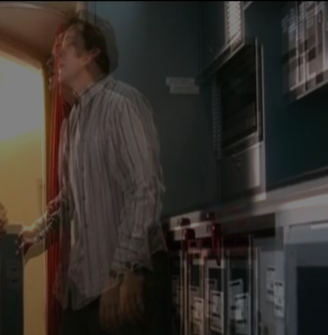
\includegraphics[width=\textwidth]{figures_3_video_body_tracking/o.png}
                \caption{\footnotesize }
                \label{fig:nonw_avg}
        \end{subfigure}
        \begin{subfigure}{0.268\textwidth}
                \centering
                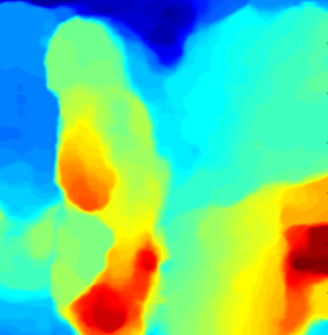
\includegraphics[width=\textwidth]{figures_3_video_body_tracking/o_mag.pdf}
                \caption{\footnotesize }
                \label{fig:nonw_flow}
        \end{subfigure}
        \begin{subfigure}{0.23\textwidth}
                \centering
                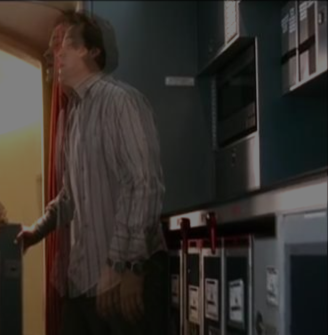
\includegraphics[width=\textwidth]{figures_3_video_body_tracking/w.png}
                \caption{\footnotesize }
                \label{fig:w_avg}
        \end{subfigure}
        \begin{subfigure}{0.23\textwidth}
                \centering
                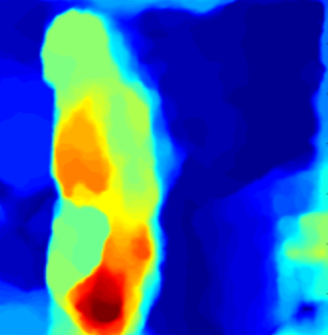
\includegraphics[width=\textwidth]{figures_3_video_body_tracking/w_mag.png}
                \caption{\footnotesize }
                \label{fig:w_flow}
        \end{subfigure}
        \caption{Results of optical-flow computation: (a) average of frame pair, (b) optical flow on (a), (c) average of frame pair after camera compensation, and (d) optical-flow on (c)}
        \label{fig:warpdemo}
\end{figure}

To obtain $f_{i+\delta}$, we must know where the frames $f_{i}$ occur in each movie. Unfortunately, this was non-trivial as the authors Sapp et al.~\cite{modec} could not provide us with the exact version of the movie that was used for creating the original dataset. Corresponding frames can be very different in multiple versions of the same movie (4:3 vs wide-screen, director's cut, special editions, etc.). We estimate the best similarity transform $S$ between $f_{i}$ and each frame $f^{m}_{j}$ from the movie $m$, and if the distance $|f_{i} - S f^{m}_{j}|$ is below a certain threshold (10 pixels), we conclude that we found the correct frame. We visually confirm the resulting matches and manually pick frames for which the automatic matching was unsuccessful (e.g. when enough feature points were not found).

\subsection{Convolutional Network}
\label{sec:conv_model_video}

As previously mentioned, the network architecture is a simple extension to the network described in Section~\ref{sec:conv_model}. The sliding window model of the new network is shown in Figure~\ref{fig:multiResPatchModel_video}, with the additional motion feature inputs. Another slight variation to the model of Section~\ref{sec:conv_model} is that not only are the input patches first normalized using Local Contrast Normalization (LCN~\cite{torch7}) for the RGB channels, we also normalize the motion features with a new normalization method we call \emph{Local Motion Normalization} (LMN). We formulate LMN as the local subtraction with the response from a Gaussian kernel with large standard deviation followed by a divisive normalization.  The result is that it removes some unwanted background camera motion as well as normalizing the local intensity of motion (which helps improve network generalization for motions of varying velocity but with similar pose). Note that the result of this stage is similar to the technique of Matsushita et al.~\cite{matsushita}, who also use Gaussian high-pass filtering on motion flow images to remove undesired camera motion when performing camera stabilization. Prior to processing through the convolution stages, the normalized motion channels are concatenated along the feature dimension with the normalized RGB channels, and the resulting tensor is processed though the same efficient sliding window network architecture as was presented in Section~\ref{sec:conv_model} and will not be replicated here for brevity.

\begin{figure}[ht]
\centering
    \includegraphics[width=\columnwidth]{figures_3_video_body_tracking/patch_model_mdr}
    \caption{Sliding-window with image and flow patches}
  \label{fig:multiResPatchModel_video}
\end{figure}

\subsection{Simple Spatial Model}
\label{sec:spatialModel}

Instead of using the spatial model from Section~\ref{sec:spatialmodel}, we will use a simplified model for the experiments in Section~\ref{chap:3_video_body_tracking_experimental} to better highlight the impact of our chosen motion features.  When the full model is used, the performance on the FLIC dataset is so high that the included motion features will have a marginal contribution to performance. We believe that on harder datasets (such as LSP and MPII) this impact will be greater, however at the time of writing we do not have access to multiple video frames for these datasets.

The core of our simplified Spatial-Model is an empirically calculated \emph{joint-mask}, shown in Fig~\ref{fig:spatialModel}(b). The joint-mask layer describes the possible joint locations, given that the supplied torso position is in the center of the mask.  To create a mask layer for body part $A$, we first calculate the empirical histogram of the part $A$ location, $x_A$, relative to the torso position $x_T$ for the training set examples; i.e. $x_{\text{hist}}=x_A-x_T$.  We then turn this histogram into a Boolean mask by setting the mask amplitude to 1 for pixels for which $p\left(x_{\text{hist}}\right) > 0$. Finally, we blur the mask using a wide Gaussian low-pass filter which accounts for body part locations not represented in the training set (but which might be present in the test set).

\begin{figure}[ht]
  \centering
    \includegraphics[width=\columnwidth]{figures_3_video_body_tracking/spatial_model}
    \caption{Simple spatial model used to mask-out the incorrect shoulder activations given a 2D torso position}
  \label{fig:spatialModel}
\end{figure}

The inclusion of this stage has two major advantages.  Firstly, as with the full graphical model from Section~\ref{sec:spatialmodel} the correct feature activation from the Part-Detector output is selected for the person for whom a ground-truth label was annotated.  An example of this is shown in Fig~\ref{fig:spatialModel}. Secondly, since the joint locations of each part are constrained in proximity to the single ground-truth torso location, then (indirectly) the connectivity between joints is also constrained, enforcing that inferred poses are anatomically viable (i.e. the elbow joint and the shoulder joint cannot be to far away from the torso, which in turn enforces spatial locality between the elbow and shoulder joints).

During test time, this joint-mask is shifted to the ground-truth torso location and the per-pixel energy from the Part-Model (section~\ref{sec:conv_model_video}) is then multiplied with the mask to produce a filtered output.  This process is carried out for each body part independently. One can view this simplified model as a star graph with the torso joint as the root and all joints as children to the torso. With weaker prior terms compared to the full spatial model from Section~\ref{sec:spatialmodel} (since the torso is only weakly coupled to joints such as the wrist and ankle), we do not expect this model to work as well but it will help disambiguate when there are multiple subjects per frame.

It should be noted that while this Spatial-Model does enforce some anatomic consistency, it does have limitations.  Notably, we expect it to fail for datasets where the range of poses is not as constrained as the FLIC dataset (which is primarily front facing and standing up poses).

%===========================================================
\chapter{Experimental Results
\label{chap:3_video_body_tracking_experimental}}

\section{Results}

Training time on the FLIC-motion dataset (3957 training set images, 1016 test set images) for the model of Section~\ref{sec:conv_model_video} is similar to the original model in Section~\ref{chap:2_body_tracking_archiecture}; approximately 12 hours. FPROP of a single image takes approximately 50ms\footnote{Analysis of our system was on a 12 core workstation with an NVIDIA Titan GPU}. For our models that use optical flow as a motion feature input,  the most expensive part of our pipeline is the optical flow calculation, which takes approximately 1.89s per image pair. We plan to investigate real-time flow estimations in the future. 

Section~\ref{sec:resultsMotionFeats} compares the performance of the motion features from section~\ref{sec:motionFeats}.  Section~\ref{sec:resultsComparison} compares our architecture with other techniques and shows that our system significantly outperforms existing state-of-the-art techniques. Note that for all experiments in Section~\ref{sec:resultsMotionFeats} we use a smaller model with 16 convolutional features in the first 3 layers. A model with 128 instead of 16 features for the first 3 convolutional layers is used for results in Section~\ref{sec:resultsComparison}. 

\subsection{Comparison and Analysis of Proposed Motion Features}
\label{sec:resultsMotionFeats}

Fig~\ref{fig:with_without_motion} shows a selection of example images from the FLIC test set which highlights the importance of using motion features for body pose detection.  In Fig~\ref{fig:with_without_motion}(a), the elbow position is occluded by the actor's sling, and no such examples exist in the training set; however, the presence of body motion provides a strong cue for elbow location.  Figs~\ref{fig:with_without_motion}(b) and (d) have extremely cluttered backgrounds and the correct joint location is locally similar to the surrounding region (especially for the camouflaged clothing in Fig~\ref{fig:with_without_motion}(d)).  For these images, motion features are essential in correct joint localization.  Finally, Fig~\ref{fig:with_without_motion}(c) is an example where motion blur (due to fast joint motion) reduces the fidelity of RGB edge features, which results in incorrect localization when motion features are not used.

\begin{figure}[ht]
  \centering
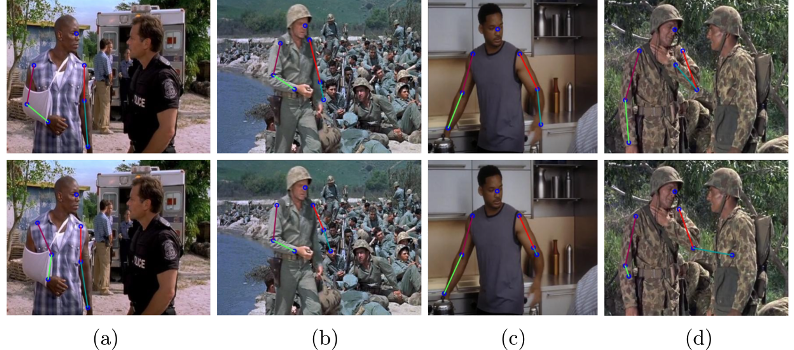
\includegraphics[width=\textwidth]{figures_3_video_body_tracking/bl_vs_mf.png}
 \caption{Predicted joint positions on the FLIC test-set. Top row: detection with motion features (L2 motion flow). Bottom row: without motion features (baseline).}
  \label{fig:with_without_motion}
\end{figure} 

Figs~\ref{fig:features_flic_results}(a) and (b) show the performance of the motion features of section~\ref{sec:motionFeats} on the FLIC-motion dataset for the elbow and wrist joints respectively. As per the evaluation of Section~\ref{chap:2_body_tracking_experimental}, we again use the criterion proposed by Sapp et al.~\cite{modec}. Surprisingly, even the simple frame-difference temporal feature improves upon the baseline result (which we define as a single RGB frame input -- i.e. the model from Section~\ref{sec:conv_model_video}) and even outperforms the 2D optical flow input (see \ref{fig:with_without_motion}(b) inset).

\begin{figure}[ht]
        \centering
        \begin{subfigure}{0.49\textwidth}
                \centering
                \includegraphics[width=\textwidth]{figures_3_video_body_tracking/best_flic_elbow_experiments.pdf}
                \caption{\footnotesize }
                \label{fig:features_flic_elbow}
        \end{subfigure}
        \begin{subfigure}{0.49\textwidth}
                \centering
                \includegraphics[width=\textwidth]{figures_3_video_body_tracking/best_flic_wrist_experiments.pdf}
                \caption{\footnotesize }
                \label{fig:features_flic_wrist}
        \end{subfigure}
        \caption{Model performance for various motion features}
        \label{fig:features_flic_results}
\end{figure}

Note that stable and accurate calculation of optical-flow from arbitrary RGB videos is a very challenging problem.  Therefore, incorporating motion flow features as input to the network adds non-trivial localization cues that would be very difficult for the network to learn internally with limited learning capacity. Therefore, it is expected that the best performing networks in Fig~\ref{fig:features_flic_results} are those that incorporate motion flow features.  However, it is surprising that using the magnitude of the flow vectors performs as well as -- and in some cases outperforms -- the full 2D motion flow. Even though the input data is richer, we hypothesize that when using 2D flow vectors the network must learn invariance to the direction of joint movement; for instance, the network should predict the same head position  whether a person is turning his/her head to the left or right on the next frame.  On the other hand, when the L2 magnitude of the flow vector is used, the network sees the high velocity motion cue but cannot over-train to the direction of the movement.

Fig~\ref{fig:analysis}(a) shows that the performance of our network is relatively agnostic to the frame separation ($\delta$) between the samples for which we calculate motion flow; the average precision between 0 and 20 pixel radii degrades 3.9\% from -10 pixels offset to -1 pixel offset.  A frame difference of 10 corresponds to approximately 0.42sec (at 24fps), and so we expect that large motions over this time period would result in complex non-linear trajectories in input space for which a single finite difference approximation of the pixel velocity would be inaccurate.  Accordingly, our results show that performance indeed degrades as a larger frame step is used.

\begin{figure}[ht]
        \centering
        \begin{subfigure}{0.45\textwidth}
                \centering
                \includegraphics[width=\textwidth]{figures_3_video_body_tracking/flic_elbow_experiment1_deltaT.pdf}
                \caption{\footnotesize }
                \label{fig:analysis_deltat}
        \end{subfigure}
        \begin{subfigure}{0.45\textwidth}
                \centering
                \includegraphics[width=\textwidth]{figures_3_video_body_tracking/flic_wrist_correction_delta-3.pdf}
                \caption{\footnotesize }
                \label{fig:analysis_camera}
        \end{subfigure}
        \caption{Model performance for (a) varying motion feature frame offsets (b) with and without camera motion compensation}
        \label{fig:analysis}
\end{figure}

Similarly, we were surprised that our camera motion compensation technique (described in section~\ref{sec:motionFeats}) does not help to the extent that we expected, as shown in Fig~\ref{fig:analysis}(b).  Likely this is because either LMN  removes a lot of constant background motion or the network is able to learn to ignore the remaining foreground-background parallax motion due to camera movement. 

\subsection{Comparison with Other Techniques}
\label{sec:resultsComparison}

Fig~\ref{fig:flic_results_video}(a) and \ref{fig:flic_results_video}(b) compares the performance of the Section~\ref{sec:conv_model_video} model with other state-of-the-art models on the FLIC dataset for the elbow and wrist joints respectively.  Our detector is able to significantly outperform all prior techniques on this challenging dataset. However, this result is not surprising since the baseline model from Section~\ref{chap:2_body_tracking_archiecture} also outperforms state-of-the-art.

\begin{figure}[ht]
        \centering
	\begin{subfigure}{\textwidth}
	\includegraphics[trim=0cm 0.6cm 1.5cm 0.6cm, clip=true, width=0.95\textwidth]{figures_3_video_body_tracking/flic_legend.pdf}
	\end{subfigure}
	\hfill
        
        \begin{subfigure}{0.45\textwidth}
                \centering
                \includegraphics[width=\textwidth]{figures_3_video_body_tracking/best_flic_elbow.pdf}
                \caption{\footnotesize }
                \label{fig:flic_elbow_video}
        \end{subfigure}
        \begin{subfigure}{0.45\textwidth}
                \centering
                \includegraphics[width=\textwidth]{figures_3_video_body_tracking/best_flic_wrist.pdf}
                \caption{\footnotesize }
                \label{fig:flic_wrist_video}
        \end{subfigure}

        \caption{Our model performance compared with our model using only flow magnitude features (no RGB image), Toshev et al.~\cite{deeppose}, Jain et al.~\cite{jainiclr2014},  MODEC~\cite{modec}, Eichner et al.~\cite{Eichner:2009:BAM}, Yang et al.~\cite{yang11cvpr} and Sapp et al.~\cite{sapp11eccv}.}
        \label{fig:flic_results_video}
\end{figure}

Note that using only motion features already outperforms~\cite{Eichner:2009:BAM, yang11cvpr, sapp11eccv}. Also note that using only motion features is less accurate than using a combination of motion features and RGB images, especially in the high accuracy region. This is because fine details such as eyes and noses are missing in motion features. Increasing the complexity of our simple spatial model by using the full model from Section~\ref{sec:spatialmodel} will improve performance further, specifically for large radii offsets.